\documentclass[a4paper, twocolumn]{article}

\usepackage[backend=biber]{biblatex}
\addbibresource{refs.bib}

\usepackage{graphicx}
\usepackage{float}
\usepackage{color}
\usepackage{url}
\usepackage{subcaption}
\usepackage{listings}
\usepackage{caption}
\usepackage{indentfirst}

\definecolor{lightgray}{gray}{0.9}



\author{Cristina Doroftei, Krisztian Szabo, Radu-Mihai Onescu}
\title{Predicting a person's country of origin by their doodles \\
    \begin{large}
        \bigskip
        Applied Artificial Intelligence elective course
    \end{large}
}

\begin{document}

\maketitle
\begin{abstract}
    In this paper we attempt to answer the question of whether or not the machine learning models available in "scikit-learn" are powerful enough to predict a person's country of origin based on their drawing style. To this end we make use of the "Quick, Draw!"\cite{quickdraw} dataset released by Google, consisting of over 50 million drawings over 345 categories. We apply different machine learning techniques and models from "scikit-learn"\cite{scikit-learn}, and compare the results. Finally, we present our conclusion, based on these findings.
\end{abstract}

\section{Introduction\label{sec:Introduction}}
The purpose of this paper is to document our journey and findings in applying the limited capabilities of "scikit-learn" to the "Quick, Draw!" dataset released by Google. This dataset is a collection of over 50 million doodles in 345 categories. It has been compiled through a browser-based online game, where players are tasked to make a series of drawings, each from a random category. The goal of the game is to succeed in creating a doodle, that is recognised by its own classifier as belonging to the requested category, all within a 20 second time limit.

We have found that virtually all papers and articles working with this dataset employ more advanced machine learning models, such as recurrent or convolutional neural networks, which are well suited to computer vision problems. In this paper we wanted to explore what can be achieved within the limitations imposed by using only the models available in "scikit-learn".

    \begin{figure}[H]
    \begin{subfigure}{.33\columnwidth}
        \centering
        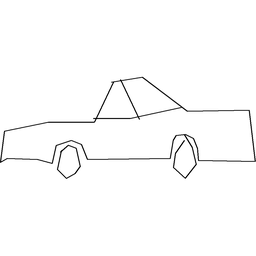
\includegraphics[width=.9\textwidth]{figures/doodle1.png}
        \caption{car}
        \label{fig:doodle1}
    \end{subfigure}%
    \begin{subfigure}{.33\columnwidth}
        \centering
        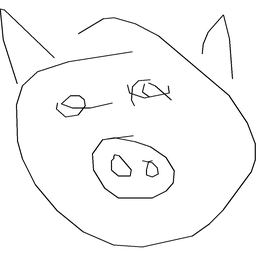
\includegraphics[width=.9\textwidth]{figures/doodle2.png}
        \caption{pig}
        \label{fig:doodle2}
    \end{subfigure}%
    \begin{subfigure}{.33\columnwidth}
        \centering
        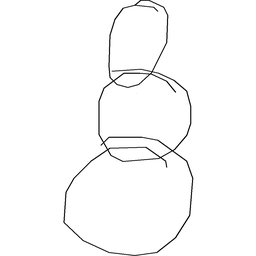
\includegraphics[width=.9\textwidth]{figures/doodle3.png}
        \caption{snowman}
        \label{fig:doodle3}
    \end{subfigure}
    \caption{Examples of doodles}
    \label{fig:doodles}
    \end{figure}

To make things interesting, we decided to attempt classifying a person's country of origin instead of the doodle's subject. It was clear from the outset that this will be challenging, and we did not necessarily expect to succeed, but we were curious as to how far we could get, if at all. There is the obvious question of whether there is enough difference in style among drawings from different countries in the first place, and secondarily whether the chosen machine learning models are able to pick up on it.

Throughout the process, we worked in an iterative way, but in this paper we present our findings in a more linear fashion. First we discuss our methods from a general standpoint. We then discuss our processes for analysing the dataset. Next we look at tuning and comparing the performance of different supervised and unsupervised learning algorithms applied to this data. Then we apply the best options to our proposed research question, and discuss our findings.

\section{Methods\label{sec:Methods}}
In the process of conducting this research we have applied quantitative methods. Methodologically speaking, we have followed the iterative approach detailed in the "Systems Development in Information Systems Research" paper by Nunamaker et al, 1990\cite{nunamaker1990systems}.

In this framework, we have repeatedly gone through the steps of data collection, preparation, interpretation, and visualisation. We have applied these in conjunction with a hypothesis-driven approach in which we work to prove or disprove our assumptions.

\section{Analysis\label{sec:Analysis}}

\subsection{Data Analysis\label{sec:Data Analysis}}
In order to start answering our main research question, the first prerequisite is to get intimately familiar with the dataset. Even though it is a cleaned and moderated dataset, it might still hide certain characteristics that could turn out to be pitfalls in our case.

We chose to work with the simplified dataset. As opposed to the raw dataset, the coordinates are normalised and the doodle is top-left aligned in a 256x256 space. In the raw dataset the coordinate spaces vary wildly based on the screen resolution of the device on which the player created the drawing. We are also giving up the time data of the drawings, but this does not affect us, as putting those datapoints to use is impractical with tools available in "scikit-learn", and thus outside of this paper's scope.

We conducted our research based on the following features of the dataset:
    \begin{itemize}
        \item word: The subject that the player was tasked to draw.
        \item countrycode: The player's country of origin, as a two letter ISO country code.
        \item recognized: Whether the game's classifier succeeded in identifying what the player is drawing within the allotted 20 seconds time limit. Filtering out the unrecognised drawings is practically always a good idea, as we were able to consistently measure a positive, albeit small, effect on classification accuracy when doing so.
        \item drawing: What the player actually drew, represented as a sequence of strokes. Each stroke is comprised, in turn, by two sequences of points of the following structure: \lbrack{}\lbrack{}x0, x1, ..., xn\rbrack{}, \lbrack{}y0, y1, ..., yn\rbrack{}\rbrack{}. For each stroke, the lengths of the two sequences are always equal.
    \end{itemize}

In some of our explorations, we have also made use of a derived datum, namely a complexity score for the drawings. We calculate it simply as the total number of points that define a drawing's strokes. This allowed us to sort the data by complexity, and observe some facts about the extremes.

    \begin{figure}[H]
        \centering
        \captionsetup{justification=centering}
        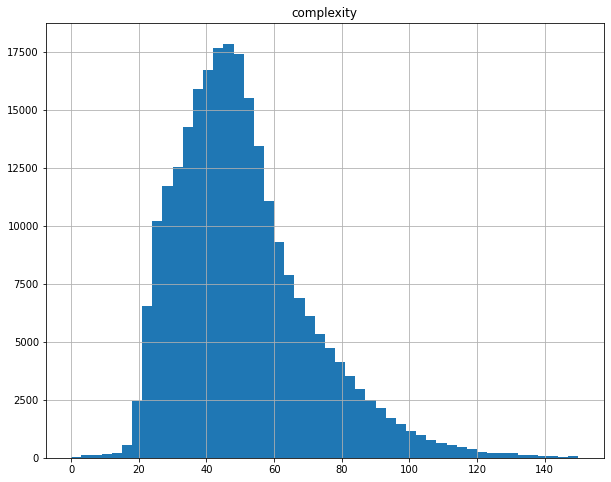
\includegraphics[width=0.4\textwidth]{figures/complexity.png}
        \caption{The complexity distribution of over 1 million drawings}
        \label{fig:complexity}
    \end{figure}

Firstly, the drawings of the lowest complexity are filled with instances that are highly ambiguous. We suspect that this phenomenon arises because the game tries to classify what the user is drawing in an eager, moment-to-moment manner. This might lead to simple lines or shapes being classified correctly simply by pure chance. This happens because prediction models will always do their best to give an answer, whereas a human would say that what the drawing represents is still inconclusive at that stage.

Secondly, among the drawings of high complexity are many instances where the player, we suspect out of frustration, simply filled the screen with senseless scribbles. These would also negatively affect the performance of models. We found that, in general, skipping the first 200 most complex doodles in any given category mitigates this issue to a satisfactory extent.

During these phases, we ran tests with loading a few random classes, or a few specific classes. From these, we either loaded all entries, a certain number of entries from the beginning of the file, a certain number of entries at random, or a certain number of the most complex entries, as was most appropriate for the task at hand. We also set up a way to ensure that we can easily extract an equal number of entries per country of origin from any given category.

The main way we explored the dataset and attempted to visually get a sense of the contents of drawings, was to render images of a few hundreds, up to a thousand of drawings. When done on a single category, it helps with finding common patterns that repeat throughout, to help distinguish it from the others. This can be taken one step further, and render such superimposed doodles for each country of origin. This would allow noticing if people from one particular country tend to draw a certain thing in a more unique way, compared to all the other countries.

    \begin{figure}[H]
    \begin{subfigure}{.33\columnwidth}
      \centering
      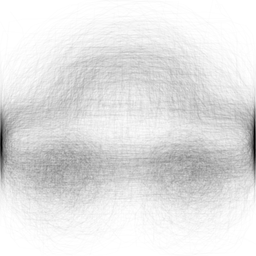
\includegraphics[width=.9\textwidth]{figures/car.png}
      \caption{cars}
      \label{fig:cars}
    \end{subfigure}%
    \begin{subfigure}{.33\columnwidth}
      \centering
      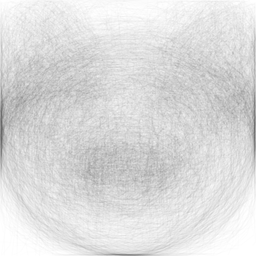
\includegraphics[width=.9\textwidth]{figures/pig.png}
      \caption{pigs}
      \label{fig:pigs}
    \end{subfigure}%
    \begin{subfigure}{.33\columnwidth}
      \centering
      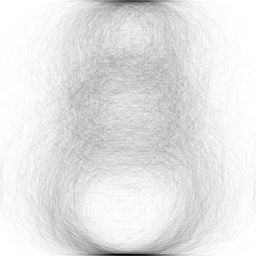
\includegraphics[width=.9\textwidth]{figures/snowman.png}
      \caption{snowmen}
      \label{fig:snowmen}
    \end{subfigure}
    \caption{1000 superimposed drawings of...}
    \label{fig:superimposed}
    \end{figure}

\subsection{Model Analysis\label{sec:Model Analysis}}
For the purposes of model analysis, selection, and tuning we chose to use 'word' (the category) as our target. As the features will stay the same, namely the columns of pixel data, this does not make a difference for the exploratory phases, before we attempt to directly answer our research question. There are a couple of main advantages to taking this approach: The differences between categories are much more obvious to our eyes, than the differences in drawing style of people from distinct countries. Another practical aspect is that it is easier to load data by category, and ensure an equal number of instances for the classes, as the dataset is already split into files according to this criterion. Keeping things simple means that we can work faster, overall, and thus maintain a shorter iteration time.

Because this dataset contains drawings as sequences of strokes defined by 2d coordinates, the question of how different ways of rendering them would affect model performance arose. To this end, we compared the performance of the same model trained on the same drawings that were rendered with different settings. We found that increasing the resolution has an inconsistent effect on model performance, but roughly a quadratic penalty on training time and memory usage. Therefore we decided to render the images to a resolution of 32x32. The width of the stroke doesn't seem to matter measurably for sensible values, i.e. as long as one makes sure that strokes don't become too thick and overlap. Drawing the lines with anti-aliasing has a measurable, small, positive impact, and because it does not affect rendering time significantly, we decided to keep using it.

Throughout the project's duration, we've consistently used an 80/20 split for training and test data, and have always applied standardisation and dimensional reduction to the data, mostly in order to optimise training time. Since we are dealing with simple black and white doodles, the resulting pixel data is fairly sparse, and this makes applying this strategy generally advantageous. On average, applying PCA reduces the number of features in half, while maintaining around 85\% of the variance.

For the purpose of model tuning, we used grid search for finding the ideal hyperparameters for each model, as applied to our particular dataset. Most of the benchmarks mentioned in this paper have been measured on a subset of the entire dataset, consisting of 40 hand-picked categories which are internally more regular (superimposing many such doodles reveals a clear pattern), and which are relatively visually distinct from each other.

\subsubsection{Unsupervised Learning\label{sec:Unsupervised Learning}}
We also explored using unsupervised learning methods to attempt automatically finding different 'archetypes', as we call them, within a given category. We noticed that in some categories one can clearly see certain distinctions for one or a small group of countries. For example, the 'power outlet' category shows some clear regional variations, brought about by the different standards for power outlets that are in use across the world.

    \begin{figure}[H]
        \centering
        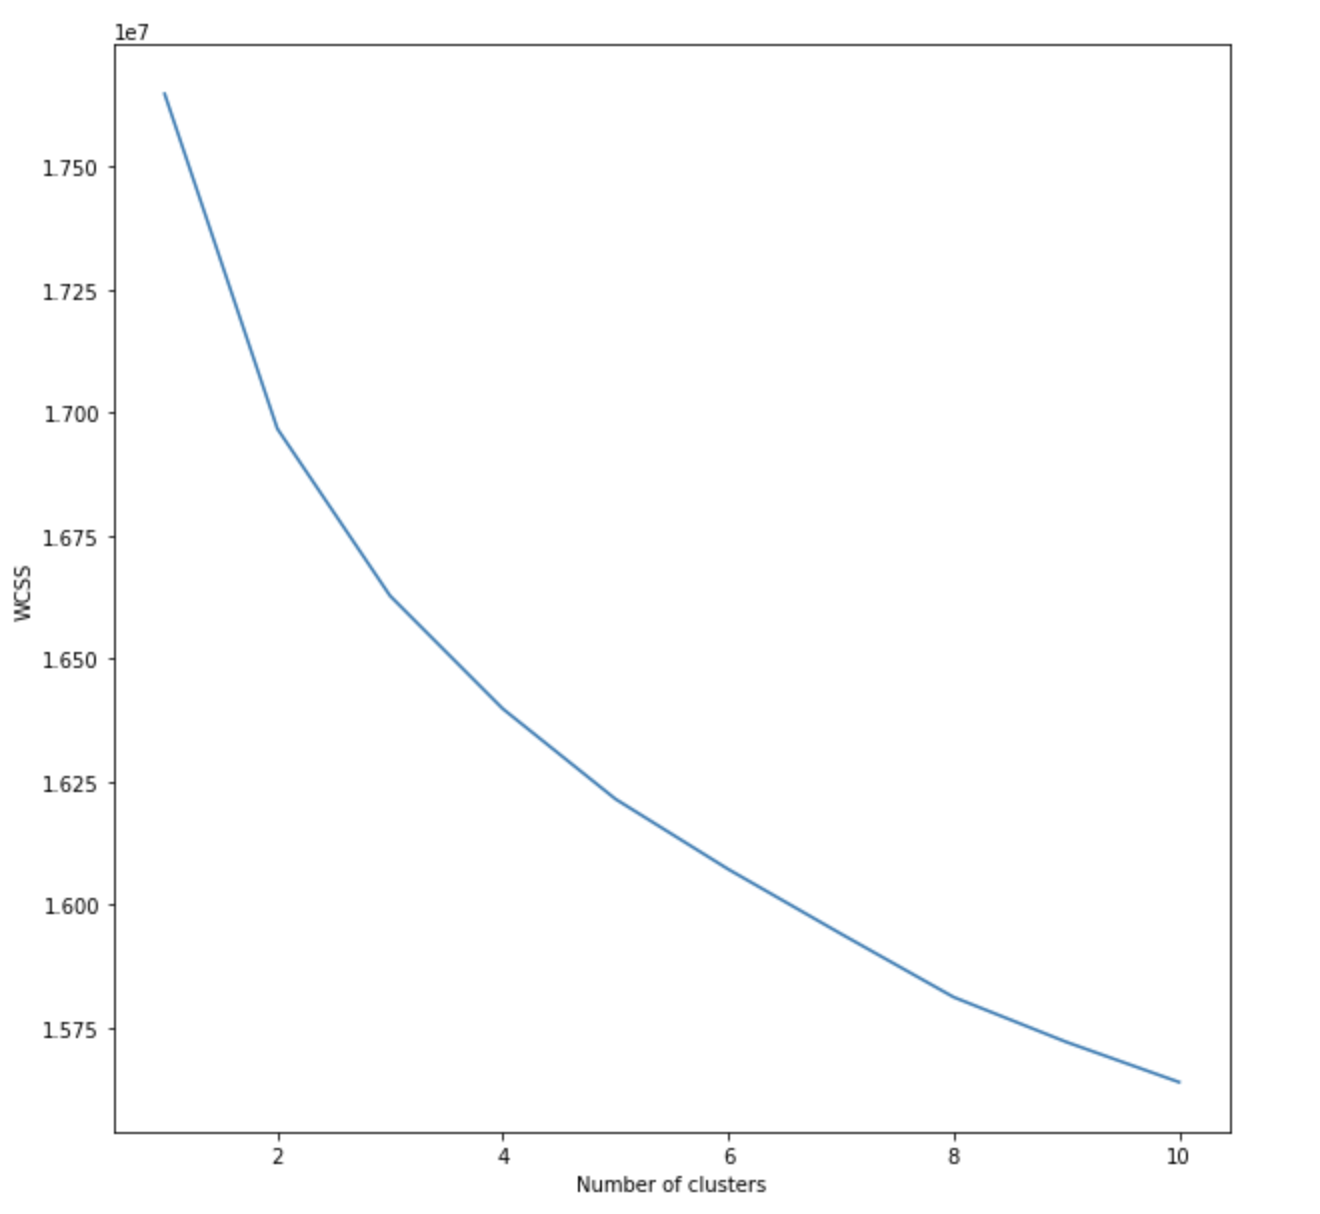
\includegraphics[width=0.4\textwidth]{figures/elbow.png}
        \caption{Elbow graph}
        \label{fig:elbow}
    \end{figure}

We tested multiple algorithms. For the ones that require a number of clusters as a hyperparameter, we tried finding a good starting value through the elbow method. Unfortunately, in the case of our dataset, for any category that we tried, the resulting graph is a smooth arc, with no clear elbow, indicating that our dataset is rather homogenous. We settled on using "KMeans", "Birch", and "Gaussian", and started with between 4 and 6 clusters per category, based on how much visual variance we could ourselves see within the given category.

To note, we also tried using methods of dimensional reduction other than PCA, and we also tried performing outlier removal, but we did not find these to make any difference.

\subsubsection{Supervised Learning\label{sec:Supervised Learning}}
For doing multi-class classification, we employed the one-vs-rest strategy, which means that our model will internally train one classifier for each class, that answers the question of how likely or not it is that a particular instance belong to the class. Comparing the answers of these internal models, the overall algorithm will answer with that class which has the highest probability.

We have tested many of the classifiers available in "scikit-learn", and from the best performing ones, we chose to work with "MLPClassifier" and "SVC" TODO add one more. While "NuSVC" and "KernelRidge" sometimes performed marginally better, they took too long to train, in the case of the former, or required too much memory during training, in the case of the latter.

\section{Findings\label{sec:Findings}}
In the case of unsupervised learning, the outcome was underwhelming. From our list of 40 curated categories, these algorithms were generally able to tease apart two archetypes. For very few of them, sometimes a weak third archetype was found. We mean weak in the sense that it had a high degree of similarity to one of the other two. This proved to be far from enough, to have any predictive power for the country of origin.

    \begin{figure}[H]
        \begin{subfigure}{.33\columnwidth}
            \centering
            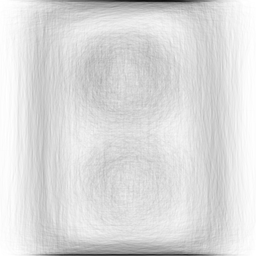
\includegraphics[width=.9\textwidth]{figures/kmeans-cluster0.png}
            \caption{Cluster 1}
            \label{fig:kmeans-cluster0}
        \end{subfigure}%
        \begin{subfigure}{.33\columnwidth}
            \centering
            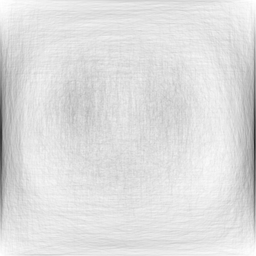
\includegraphics[width=.9\textwidth]{figures/kmeans-cluster1.png}
            \caption{Cluster 2}
            \label{fig:kmeans-cluster1}
        \end{subfigure}%
        \begin{subfigure}{.33\columnwidth}
            \centering
            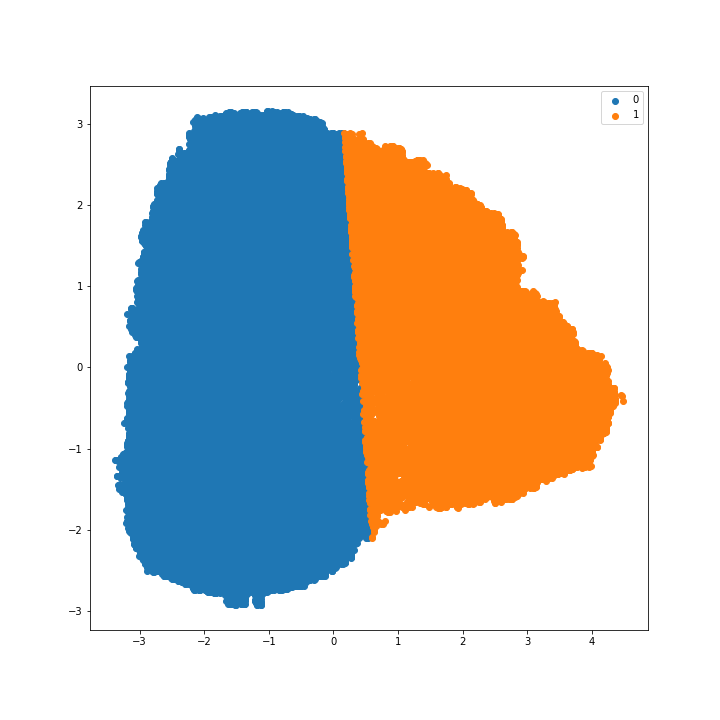
\includegraphics[width=.9\textwidth]{figures/kmeans-plot.png}
            \caption{plot}
            \label{fig:kmeans-plot}
        \end{subfigure}
        \caption{KMeans}
        \label{fig:clustering}
    \end{figure}

In the case of supervised learning, on the other hand, the accuracy for classifying 40 categories is in the 50-60\% range, much higher than what would be expected from random chance, which works out to 2.5\%. We consider this good performance, especially keeping in mind the inherent ambiguity in the dataset, as previously discussed.

    \begin{figure}[H]
        \centering
        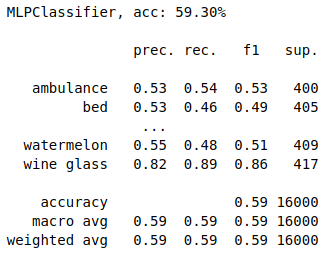
\includegraphics[width=0.4\textwidth]{figures/supervised.png}
        \caption{Category classifier}
        \label{fig:supervised}
    \end{figure}

But when we switched our target from 'word' to 'countrycode', we found that the algorithms lost much of their predictive power. And this despite the fact that for any given category there's usually only about 15-25 countries of origin with a high enough number of instances to train on. For most classes, the accuracy was barely above random chance, with a few classes, usually 2-3, that were more easily identified, with an accuracy up to 4 times higher than random chance.

    \begin{figure}[H]
        \centering
        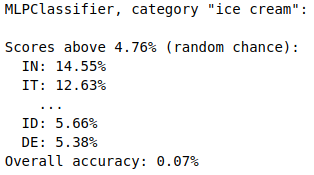
\includegraphics[width=0.4\textwidth]{figures/supervised2.png}
        \caption{Country classifier}
        \label{fig:supervised2}
    \end{figure}

\section{Conclusion\label{sec:Conclusion}}
The performance we were able to obtain from the models available in "scikit-learn" is not enough to successfully predict a person's country of origin based on their drawing style. The unsupervised learning models performed abysmally, far from what we would need for these purposes. Even in the case of supervised learning, which we proved can work decently on this kind of data in general, we did not achieve a high enough accuracy to give us enough predictive power. We have initially envisioned finding a series of categories, with high enough predictive power for a high enough number of countries of origin, such that asking a person to draw several doodles from specific categories would progressively increase our confidence in a particular answer. Based on our findings, we have concluded that this is simply not possible due to the lack of predictive power with respect to the country of origin. This level of performance might allow a series of such models to tentatively suggest that a user might be from a particular country out of a small list, but this is a far cry from the performance needed to predict the country of origin for any random person from across the globe.

It remains an open question whether this is at all possible with more advanced algorithms. From our work, we can clearly conclude that the tools available in "scikit-learn" are simply not powerful enough to achieve this goal. Whether there is enough variation by country in the dataset to begin with, and whether this can be detected with more advanced models, will remain two questions that we cannot answer at all based on the work in this paper.

\printbibliography

\end{document}
